\chapter{Case Study}
In a nutshell, curriculum learning means "training from easier data to harder data" \cite{Wang2020}. More specifically the
core idea is to "start small" \cite{ELMAN199371}, train the machine learning model with easier subtasks, to then gradually increase
the difficulty level of subtasks until the whole training dataset is used.\\
Bearing in mind the strategy of training from easier to harder data, to design such a curriculum idea 
(i), what kind of training data is supposed to be easier than other data, (ii) and when is appropriate to present more harder
data for training - and how much more - must necessarily be decided.
Technically, those 2 issues can be abstracted in the concepts of a Difficulty Measurer, that decides the "easiness"
of each data instance to start the training process from, and a Training Scheduler, that rules the sequence of data subsets during 
the whole training process \cite{Wang2020}.
Therefore, Difficulty Measurer together with Training Scheduler constitute a general framework for curriculum design,
as illustrated in Figure ~\ref{fig:CLdesign}.
\begin{figure}[h]
    \begin{center}
        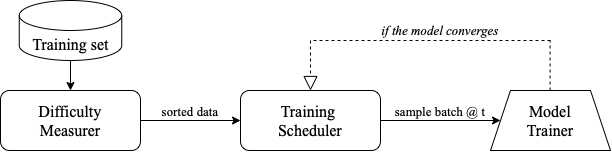
\includegraphics[width=0.55\textwidth]{/Users/carmenarmenti/Desktop/Thesis document/images/predefinedCL.png}
        \caption{\label{fig:CLdesign}Predefined Curriculum Design.}
    \end{center}
\end{figure}
First of all, the Difficulty Measurer sorts all the training examples from the easiest 
to the hardest and passes them to the Training Scheduler. Then, at each training epoch \textit{t}, the Training Scheduler
samples a batch of training instances from the easier subset and give them to Model Trainer for training.\\
As training epochs increase, the Scheduler decide qhen to sample from more harder data, generally until uniform sampling
from the whole training set. This schedule either depends on the training loss feedback from the Model Trainer, or on some other
parameters that implies that the model would deverge, if left to training for more epochs.\\
A distinction between \textbf{predefined CL} and \textbf{automatic CL} must be clarified. The first refers to the framework
where both the Difficulty Measurer and Training Scheduler are defined by human prior knowledge, thus with no data-driven
algorithms involved; the latter instead, if any - or both - of the components are designed by data-driven algorithms.\\
Usually, the power of introducting Curriculum into Machine Learning depends on how the curriculum for specific
applications and dataset is designed. Due to this, Difficulty Measurers often relies on the data
characteristics of specific tasks, and most of them are defined by complexity, diversity, or noise estimation
definitions.\\

We adopted the most popular discrete scheduler, known as \textit{Baby Step}, where the complexity of the training
data needs to be gradually increasing. Due to this a reliable metric to split the initial dataset of each task needed to be defined.
This approach distributes the sorted data into buckets, from easy to hard, according to the metric and starts training with the easiest bucket. 
Starting from the easiest bucket, after a fixed number of training epochs or convergence, the subsequent bucket is merged
into the current training subset - main characteristic of \textit{Baby Step} approach.
Finally, once all the buckets are merged and used, the
training process either stops or continues several extra epochs.\\
Note that, at each epoch the scheduler shuffles the current bucket and samples mini-batches for training.\\

However, before testing curriculum learning approach, we thougth it was strictly necessary reproducing - in the case 
of bug-fixing task - or conducting -  within the framework of the other 2 tasks - the experiment on the modelbase.\\
We worked with a neural network whose configuration is composed by 1-layer bidirectional Encoder, 2-layer Attention 
Decoder both with 256 units, embedding size of 512, and LSTM RNN cells.\\

In this chapter, we present how we applied Curriculum Learning to some of Software
Engineering tasks, i.e. \textit{bug-fixing}, \textit{code summarization}, and \textit{log generation}
tasks. \\
For each of the tasks considered, the following aspects are described thoroughly:
\begin{itemize}
    \item \textbf{Dataset characteristics}: the datasets used are composed by a couple, where the first element is the source of the training, while the second is the target;
    \item \textbf{Difficulty Measurer}: a measure to sort the datasets' instances is needed, each task was experimented with a different metric; 
    \item \textbf{Training Scheduler}: sequence of data subsets are presented to the model following a training schedule.
\end{itemize}


The goal of this study is to asses whether Neural Machine Translation, combined with the Curriculum Learning approach, 
can be used for the tasks experimented. In the following section, the design of our study is described in detail.

% ADDITIONS
% need to add information about training on baseline, i.e. in the introduction you must explain that before trying
% to test the CL approach 

\section{Neural Machine Translation}
The experimented models are based on an Recurrent Neural Network (RNN) Encoder-Decoder
architecture with attention mechanism, frequently used in Neural Machine Translation. This kind of model is composed by two
dominant components:

\begin{itemize}
    \item a RNN Encoder, which encodes a sequence of terms \textbf{x} into a vector representation;
    \item a RNN Decoder, which decodes the vector representation into another sequence of terms \textbf{y}.
\end{itemize}

The model learning is based on a conditional distribution, where the output sequence of terms is conditioned
by the input sequence: \(P(y_1,...,y_m|x_1,...,x_n)\), where \(m\) and \(n\) not necessarly have to have the same length.
The Encoder takes as input a sequence \textbf{x}\(= (x_1,...,x_n)\) and produces
a sequence of states \textbf{h}\(= (h_1,...,h_n)\). The framework relies on a bi-directional
RNN Encoder, which is composed by a backward and a forward RNN, where both are able to create representations taking into account
past and future inputs. Specifically, each state \(h_i\) is the concatenation of the states produced by 
the two RNNs when reading the sequence not only in a forward but also in a backward manner.\\
The RNN Decoder computes the probability of a target sequence \textbf{y}\(= (y_1,...,y_n)\) given \textbf{h}. The probability
of each output term \(h_i\) is computed based on:
\begin{itemize}
    \item the recurrent state \(s_i\) in the Decoder;
    \item the previous \(i - 1\) terms \((y_1,...,y_i-1)\);
    \item a context vector \(c_i\), which constitutes the attention mechanism.
\end{itemize}
The vector \(c_i\) is a weighted average of the states in \textbf{h}, where the weights associated 
to each state allow the model to pay more attention to some parts of the input sequence than to others:
\[c_i = \sum_{t=1}^n a_it h_t\]
Precisely, the weigth \(a_it\) defines how much the model should take into consideration the term of the sequence in input \(x_i\)
when predicting the target term \(y_t\). Encoder and Decoder are simultaneously trained - instead of sequentially - by minimizing
the negative log likelihood of the target terms, using stochastic gradient descent.
The configuration used by the neural network is composed by 1-layer bidirectional Encoder, 
2-layer Attention Decoder both with 256 units, embedding size of 512, 
and LSTM RNN cells. Bucketing and padding was used to deal with the variable length of the sequences.


\section{Canonical Training}



\section{Training with Curriculum Learning}

...

\section{Bug fixing task}
In this section the way how the bug fixing task is applied in the CL approach is presented.

\subsection{Dataset characteristics}
The dataset used to train the NMT model is the union between \textit{small} and \textit{medium} method-level datasets
used by Tufano \textit{et al.} \cite{Tufano2019}. The reason for this specific choice was firstly
to avoid any type of context dependance, secondly to achive a reasonable number of training instances.
Each instance of the dataset is a pair $(m_b, m_f)$, where $m_b$ is a buggy code component and $m_f$ is the
corresponding fixed code. These BFPs were used to train the NMT model, allowing it learning the translation
from the buggy to the fixed method, thus being able to generate fixing patches.

\begin{lstlisting}[language=Java, caption={Buggy code},label={lst:buggy1}, mathescape=true, breaklines=true]{Name}   
    public void METHOD_1 ( TYPE_1 VAR_1 ) { VAR_2 . METHOD_2 ( VAR_3 ) ; ( VAR_4 ) ++ ; METHOD_3 ( ) ; } 
\end{lstlisting}


\begin{lstlisting}[language=Java, caption={Fixed code},label={lst:fixed1}, mathescape=true, breaklines=true]{Name}
    public void METHOD_1 ( TYPE_1 VAR_1 ) { if ( VAR_2 . METHOD_2 ( VAR_3 ) ) { ( VAR_4 ) ++ ; METHOD_3 ( ) ; } }
\end{lstlisting}

%\noindent\begin{minipage}{.45\textwidth}
%\begin{lstlisting}[language=Java, caption={Buggy code},label={lst:buggy1}, mathescape=true, breaklines=true, frame=tlrb]{Name}
%    public void METHOD_1 ( TYPE_1 VAR_1 ) 
%    { VAR_2 . METHOD_2 ( VAR_3 ) ; 
%    ( VAR_4 ) ++ ; METHOD_3 ( ) ; }
%\end{lstlisting}
%\end{minipage}\hfill
%\begin{minipage}{.45\textwidth}
%\begin{lstlisting}[language=Java, caption={Fixed code},label={lst:fixed1}, mathescape=true, breaklines=true, frame=tlrb]{Name}
%    public void METHOD_1 ( TYPE_1 VAR_1 ) 
%    { if ( VAR_2 . METHOD_2 ( VAR_3 ) ) 
%    { ( VAR_4 ) ++ ; METHOD_3 ( ) ; } }
%\end{lstlisting}
%\end{minipage}
%%%%%%%%%%%%%%%%%%%%%%%
% TODO: Insert instance ex.
%%%%%%%%%%%%%%%%%%%%%%%

%%% DATASET DESCRIPTION
\subsection{Difficulty Measurer}
As stated above, a difficulty measurer definition is the core element of the approch implemented.\\
For the task at issue here the \textbf{Levenshtain distance} was used as metric. The \textit{Levenshtein distance}, also known as the \textit{edit distance}, 
was introduced by Vladimir Levenshtein in 1965 \cite{Levenshtein_SPD66}. It is a string metric for measuring difference between two sequences, specifically the number of insertions, deletions, and substitutions
required to transform one string into the other. However, the distance we used for our experiments was token based, thus the granularity is word based instead of being single-character based.\\
Defined the measure, the distance between buggy and fixed method for each of the BFPs was computed and we observed the data distribution; then we used the quartiles' values to divide the initial dataset in multiples
smaller datasets, where each of these represents a different level of difficulty.\\
By doing so, we clearly obtained 4 level of difficulty; thus we defined an incremental difficulty criteria to feed the model with: 
the bug-fixing training scheduler described in Section ~\ref{scheduling-bf}.

%%%%%%%%%%%%%%%%%%%%%%%
% TODO: Insert data distribution figure
%%%%%%%%%%%%%%%%%%%%%%%

\subsection{Training Scheduler}
\label{scheduling-bf}
The \textbf{training scheduler} decides the sequence of data subsets throughout the training process based
on the judgment from the difficulty measurer. As mentioned in the introduction of this chapter, Baby Step approach switches to the next difficulty level
as soon as the model converges on the previous one.\\ 
In the bug-fixing task, the scheduler adjusts
the training data subsets based on an early stopping criterion: after a fixed number of steps
early stopping is run and it considers the model as being converging if the loss value
does not improve after 5K steps.

To guide the selection of the best configuration, we used the loss function computed on the validation set
and not on the test set, while the results are computed on the test set.

\section{Code summarization task}
Automatic source code summarization is the task of generating short natural language description 
for source code \cite{Leclair2020}. The idea is that a brief description allows programmers to understand
what a chunk of code does and what is the purpose of the program by and large, without necessarily read the code 
itself.\\
In this section CL the application of Curriculum Learning is applied to code summarization task.

\subsection{Dataset characteristics}
The training dataset used to test this software engineering task, is a subset of the data set of 2.1 million 
Java method-comment pairs used by LeClair \textit{et al} \cite{Leclair2020}. A random sample of 200K instances was picked from
the initial dataset; evaluation and test datasets, however, were used as-is. The scope of the training here 
was to make the model able to learn how to summarize pieces of code, starting from a sequence of tokenized methods.

\begin{lstlisting}[language=Java, caption={Function},label={lst:buggy1}, mathescape=true, breaklines=true]{Name}
    protected String creatorName() {
        return Texts.getText("solver");
    }
\end{lstlisting}

\begin{lstlisting}[language=Java, caption={Comment},label={lst:fixed1}, mathescape=true, breaklines=true]{Name}
    //Gives the name of this solver as used to tag new solutions.
    //@return the name of this solver
\end{lstlisting}


%%%%%%%%%%%%%%%%%%%%%%%
% TODO: Insert instance ex.
%%%%%%%%%%%%%%%%%%%%%%%

\subsection{Difficulty Measurer}
In Natural Language Processing tasks the \textbf{sentence lenght} intuitively expresses the complexity 
of a sentence. However, instead of focusing on the source of the couple, for this task we decided to sort out the subdatasets computing the
difficulty measure on the target, namely the lenght of each method's comment. 
Once obtained the lenghts, accordingly to the data distribution we took advantage of the quartiles obtained to split the intial dataset in 4 smaller 
buckets. 
\begin{figure}[h!]
    \begin{center}
        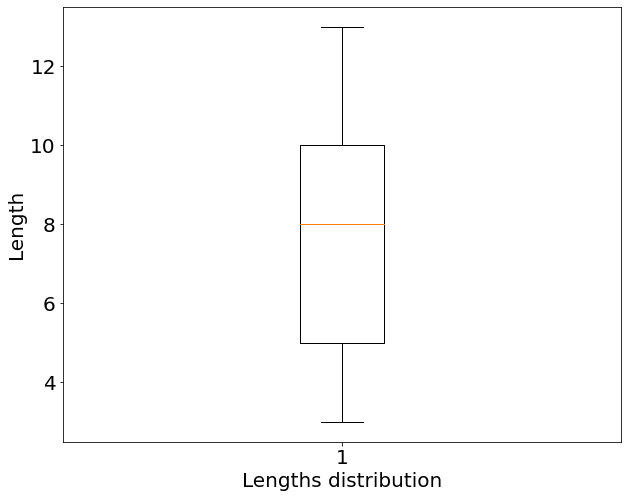
\includegraphics[width=0.35\textwidth]{/Users/carmenarmenti/Desktop/Thesis document/images/boxplot-length.png}
        \caption{\label{fig:CSdistribution}Code summarization task: data distribution.}
    \end{center}
\end{figure}
%%%%%%%%%%%%%%%%%%%%%%%
% TODO: Insert data distribution figure
%%%%%%%%%%%%%%%%%%%%%%%

\subsection{Training Scheduler}
Similarly to what happens in bug-fixing task, the training scheduler decides to sample from more harder data only when the model converges on the 
previous easier bucket. The convergence is assessed after a fixed number of epochs, after which early stopping with patience of 5 epochs
is run. Once the model converget on the first bucket, the training proceeds on the second and so forth. 

\section{Log generation task}
Inserting log messages is a practice broadly used and decide where to inject log statements, what information to report through it, 
and at which log level is as hard as it is crucial \cite{Mastropaolo2022}. In the following section Curriculum Learning is applied
at log generation task.

\subsection{Dataset characteristics}
The dataset for this task is composed by couple of methods, where the source is the method without the log statement,
the target instead has not only the log statement but also the log message.\\
Those couples where used to train the model to generate and inject log statements in Java code.


\noindent\begin{minipage}{.45\textwidth}
\begin{lstlisting}[language=Java, caption={Method},label={lst:buggy1}, mathescape=true, breaklines=true]{Name}
    public CsvDestination setPath ( final String path ) 
    { if ( csvFile != null ) 
    { throw new UnsupportedOperationException ( ""Changing the value of path after opening the destination is not allowed."" ) ; } 
    if ( outputChannel != null ) 
    { try 
    { outputChannel . close ( ) ; 
    outputChannel = null ; } 
    catch ( final IOException e ) { } } 
    this . path = path ; 
    return this ; }
\end{lstlisting}
\end{minipage}\hfill
\begin{minipage}{.45\textwidth}
\begin{lstlisting}[language=Java, caption={Method + log statement},label={lst:fixed1}, mathescape=true, breaklines=true]{Name}
    public CsvDestination setPath ( final String path ) 
    { if ( csvFile != null ) 
    { throw new UnsupportedOperationException ( ""Changing the value of path after opening the destination is not allowed."" ) ; } 
    if ( outputChannel != null ) 
    { try 
    { outputChannel . close ( ) ; 
    outputChannel = null ; } 
    catch ( final IOException e ) 
    { log . error ( String . format ( ""Could not close file channel with CSV results for file %s."" , csvFile ) , e ) ; } } 
    this . path = path ; 
    return this ; }
\end{lstlisting}
\end{minipage}

%%%%%%%%%%%%%%%%%%%%%%%
% TODO: Insert instance ex.
%%%%%%%%%%%%%%%%%%%%%%%

\subsection{Difficulty Measurer}
Given the dataset at our dispose we choose as difficulty measurer the 
complexity of the instruction set in program execution tasks. More specifically we 
computed \textbf{cyclomatic complexity} through Lizard tool \cite{lizard}. Cyclomatic complexity
is a quantitative software metric developed by Thomas J. McCabe in 1976 used to indicate
the complexity of a program.  
It measures the number of linearly-independent paths through a program module. 
The measure is computed using the control-flow graph of the program where
the nodes of the graph correspond to sets of commands of a program, and
a directed edge connects 2 nodes if the second command might be executed
immediately after the first command. It can be applied to individual functions,
modules, methods or classes within a program. We decided to compute it on each of
the source methods.\\
It must be said that from the initial dataset were removed 397 instances whose
cyclomatic complexity was 0. Decided and computed the difficulty measure
for each instance, the dataset was ready to be used by the training scheduler.

%%%%%%%%%%%%%%%%%%%%%%%
% TODO: Insert data distribution figure
%%%%%%%%%%%%%%%%%%%%%%%

\subsection{Training Scheduler}
Once again we observed the data distribution and considered the 3 quartiles
to divide the whole dataset in 4 subsets. Each of those represented a differen level of difficulty.\\
As soon as the model converged on the current bucket, BLEU values after each epoch were considered,
and early stopping was applied. We took the best model before divergence to restart the training 
on the following bucket. 


%%%%%%%%%%%%%%%%%%%%%%%
%RANDOM NOTES: 
%to use to sort the instances at dispose
%Only after this choice the initial dataset
%was divided in multiple smaller datasets For the task at issue here 
%the instances of th

%Once defined the measure, we were able to divide the initial dataset in smaller datasets so as to define 
%an incremental difficulty criteria to feed the model with. 

%For each of the task considered, a different metric to split the datasets was used.
%%%%%%%%%%%%%%%%%%%%%%%




